\documentclass{scrartcl}
% Packages
\usepackage{hyperref}
\usepackage{tikz}
\usepackage{amsmath}
\usepackage{pifont}
\usepackage{mathrsfs}
\usepackage{amssymb}
\usetikzlibrary{arrows.meta, positioning}

\definecolor{darkgreen}{rgb}{0.0, 0.5, 0.0}

\newcommand{\tto}{\twoheadrightarrow}


\title{Summer 2024 Report}
\author{Sam Arkle}
\date{\today}

\begin{document}

\maketitle

\section{Introduction}
This is a report on the progress I have made during the summer of 2024 working with Dr. Polonsky \footnote{Assisstant Professor, Department of Computer Science, Appalachian State University.}. I have been writing on the topic of relations, working primarily from Term Rewriting Systems (TeReSe) \footnote{(Term Rewriting Systems. (2003). United Kingdom: Cambridge University Press.)}.
The objective of this work has been to both develop a formal understanding of relations and to build a library in Agda \footnote{\href{https://github.com/DrPolonsky/LAM/tree/main/Relations}{Github repository for this project's code}} that will be used as a foundation to further work in theoretical computer science.
\\
I have been focussed on Chapter 1 of TeReSe which covers abstract reduction systems (ARS) as well as the appendix (sections 1-3) which provides the necessary mathematical background for the rest of the book (e.g. relations, ordinals, inductive definitions and the Knaster-Tarski lemma). Where the book has made use of classical logic I have investigated the possibility of using constructive alternatives.

\section{Relations}

\subsection{Well-foundedness}
\textcolor{red}{Talk about the different types of wellfoundedness, starting with the one given in the book, the reason for thinking it is classical and not constructive, and provide an image showing the relation between the notions of wellfoundedness we have. Talk about future work in this area.}
\\
To date we have investigated the differences between four distinct notions of well-foundedness. The make clear the difference between these distinct notions of well-foundedness we first present the following defintiions for a given relation $R$.
\begin{enumerate}
    \item \textit{Accessible:} An element $x$ is \textit{R-accessible} if all elements that have an $R$ reduction to $x$ are themselves \textit{R-accessible}.  
    \item \textit{Inductive predicate:} A predicate $\varphi$ is an inductive predicate if $\varphi \, x$ is true whenever $\varphi$ is true for all elements that have an $R$ reduction to $x$.
    \item \textit{Minimal element:} An element $x$ is minimal for a given predicate $\varphi$ if $\varphi \, x$ is true and no other element for which $\varphi$ holds has an $R$ reduction to $x$. 
    \item \textit{Decreasing:} A sequence $s$ is decreasing if every $R$ reduction decreases the size of $n$ (where $n \in \mathbb{N}$).   \textcolor{red}{bad defn. Improve.}
\end{enumerate}
With the above definitions established we define the notions of well-foundedness we have been investigating. For a given relation $R$:
\begin{enumerate}
    \item \textit{R} is well-founded if every element is \textit{R}-accessible.
    \item \textit{R} is well-founded if every inductive predicate is universally true.
    \item \textit{R} is well-founded if every non-empty predicate has a minimal element with respect to $R$.
    \item \textit{R} is well-founded if every sequence contains a non-decreasing index.
\end{enumerate}
Further, we explored weaker variants of these notions of well-foundedness:
\begin{enumerate}
    \item \textit{R} is well-founded if every element is $\lnot \lnot$  \textit{R}-accessible.
    \item \textit{R} is well-founded if for every inductive predicate $\varphi$, $\lnot \lnot \varphi$ is universally true.
    \item \textit{R} is well-founded if it is not not the case that every non-empty predicate has a minimal element with respect to $R$. \textcolor{red}{is there a better way to express this double negation in english?} 
    \item \textit{R} is well-founded if there is no infinite $R$-decreasing sequence (this is the definition of well-foundedness found in TeReSe).
\end{enumerate}

The following graphic illustrates the implications we have found between these definitions and those we are still seeking to find. Green arrows indicate that one definition implies another, red arrows indicate that we believe an implication should be possible but we have not yet found it.

\begin{center}
  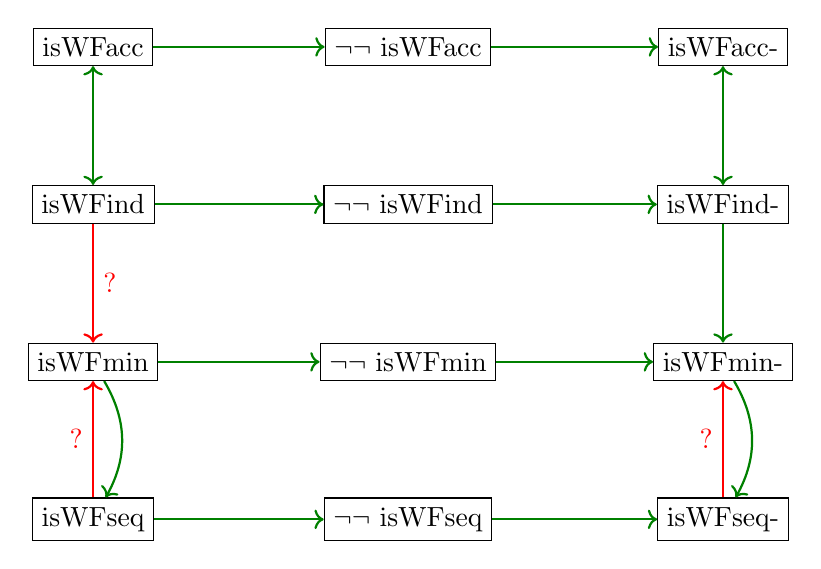
\begin{tikzpicture}[node distance=2cm, auto]
    % Standard definitions
    \node (std1) [draw] {isWFacc};
    \node (std2) [below of=std1, draw] {isWFind};
    \node (std3) [below of=std2, draw] {isWFmin};
    \node (std4) [below of=std3, draw] {isWFseq};
    
    % Double negation definitions
    \node (dn1) [right of=std1, xshift=2cm, draw] {$\lnot \lnot$ isWFacc};
    \node (dn2) [right of=std2, xshift=2cm, draw] {$\lnot \lnot$ isWFind};
    \node (dn3) [right of=std3, xshift=2cm, draw] {$\lnot \lnot$ isWFmin};
    \node (dn4) [right of=std4, xshift=2cm, draw] {$\lnot \lnot$ isWFseq};
    
    % Weaker definitions
    \node (weak1) [right of=dn1, xshift=2cm, draw] {isWFacc-};
    \node (weak2) [right of=dn2, xshift=2cm, draw] {isWFind-};
    \node (weak3) [right of=dn3, xshift=2cm, draw] {isWFmin-};
    \node (weak4) [right of=dn4, xshift=2cm, draw] {isWFseq-};
    
    % Arrows
    \draw[->, thick, darkgreen] (std1) -- (dn1);
    \draw[->, thick, darkgreen] (dn1) -- (weak1);
    \draw[<->, thick, darkgreen] (std1) -- (std2);
    \draw[->, thick, darkgreen] (std2) -- (dn2);
    \draw[->, thick, darkgreen] (dn2) -- (weak2);
    \draw[<->, thick, darkgreen] (weak1) -- (weak2);
    \draw[->, thick, red] (std2) -- (std3) node[pos=0.5, right, red] {?};
    \draw[->, thick, darkgreen] (std3) -- (dn3);
    \draw[->, thick, darkgreen] (dn3) -- (weak3);
    \draw[->, thick, darkgreen] (weak2) -- (weak3);
    \draw[->, thick, darkgreen, bend left] (std3) to (std4);
    \draw[->, thick, darkgreen, bend left] (weak3) to (weak4);
    \draw[->, thick, darkgreen] (std4) -- (dn4);
    \draw[->, thick, darkgreen] (dn4) -- (weak4);
    \draw[->, thick, red, bend left] (std4) -- (std3) node[pos=0.5, left, red] {?};
    \draw[->, thick, red, bend left] (weak4) -- (weak3) node[pos=0.5, left, red] {?};
  \end{tikzpicture}
\end{center}

  
  
  As future work we want to know whether the missing implications can be found, or what the minimal additional requirements are for making those implications.

\subsection{Definitions}
\textcolor{red}{Go through some of the main definitions formalised from Terese, focussing on where we have used constructive alternatives to the classically given definitions
Could talk here about omega bounded stuff too!}

The most interesting work we have carried out in investigating Chapter 1 of TeReSe has resulted from trying to provide constructive proofs for Newman's lemma, the Knaster-Tarski lemma, Theorem 1.2.2 and Theorem 1.2.3. Before exploring those proofs the following definitions are essential.
\begin{itemize}
  \item \textit{ARS:} An abstract reduction system (ARS) is a framework which we use to explore reduction relations on a set of objects.  
\end{itemize}
Throughout these definitions we use $A$ to denote the set which contains all the objects that can be reduced and $\to$ to denote a binary relation on $A$. This relation represents the reduction process. For example, if we let $\to$ be the relation of being 'less than' ($<$) then $4 \to 2$. \textcolor{red}{Right?}

We use $\to$ for a single-step reduction and $\tto$ for a multi-step reduction.

\begin{itemize}
  \item \textit{Weakly confluent:} A reduction relation is weakly confluent (AKA weakly Church-Rosser (WCR)) if all single-step reductions from a given element can always converge via multi-step reductions to some common reduct. 
\end{itemize}
\begin{center}
  \begin{tikzpicture}[node distance=2cm, auto]
    % Nodes
    \node (top) {a};
    \node (left) [below left of=top] {b};
    \node (right) [below right of=top] {c};
    \node (bottom) [below of=top, yshift=-1cm] {d};
  
    % Arrows
    \draw[->] (top) -- (left);
    \draw[->] (top) -- (right);
    \draw[->>] (left) -- (bottom);
    \draw[->>] (right) -- (bottom);
\end{tikzpicture}
\end{center}

\begin{itemize}
  \item \textit{Confluent} A reduction relation is confluent (AKA Church-Rosser (CR)) if all multi-step redctions from a given element can always converge via multi-step reductions to some common reduct.
\end{itemize}
\begin{center}
  \begin{tikzpicture}[node distance=2cm, auto]
    % Nodes
    \node (top) {a};
    \node (left) [below left of=top] {b};
    \node (right) [below right of=top] {c};
    \node (bottom) [below of=top, yshift=-1cm] {d};
  
    % Arrows
    \draw[->>] (top) -- (left);
    \draw[->>] (top) -- (right);
    \draw[->>] (left) -- (bottom);
    \draw[->>] (right) -- (bottom);
\end{tikzpicture}
\end{center}

\subsubsection{Strongly Normalizing}
\begin{center}
    In TeReSe: $a \in A$ is \textit{strongly normalizing} if every reduction sequence starting from $a$ is finite. The reduciton relation $\rightarrow$ is \textit{strongly normalizing} (SN) if every $a \in A$ is strongly normalizing.
\end{center}
Go through different proofs Here

\subsection{Newmans lemma}
What it is and the different definitions again

\subsection{}

\section{Notes from 08.29}
 
\begin{enumerate}
  \item Try to ``fix'' CP by changing $R$ into $R^r$
  \item Finish formulating the ``compactness property".  Two candidates:
  \begin{itemize}
    \item ``Every cocone for a given infinite sequence loops back to some point in the sequence"
    \item ``If an $R^*$-sequence has a cocone then it's constant after some point on.''
  \end{itemize}
  \item Add the definition of "recurrent element"
\end{enumerate}

\section{09.05}
\begin{enumerate}
  \item done: WN, UN, RP imply SN (classical)
  \item need: omega bounded and RP implies SN (classical)
  \item need: omega bounded and RP implies SN (constructive)
  \item do we need $s_0 \to^* s_c$ in the proof?
  \item is $\omega$-bounded implied by WN and the following confluence property:
  $a \to^* n \in NF$, and $a \to b$ then $b \to^* n $.
  \item Remark before 1.2? (Exercise 1.3.21)
  \item Make the first argument to "being a normal form" implicit?
\end{enumerate}

\newcommand{\RP}{\mathsf{RP}}
\newcommand{\NF}{\mathsf{NF}}
\newcommand{\UN}{\mathsf{UN}}
\newcommand{\UNto}{\mathsf{UN}{\to}}
\newcommand{\SN}{\mathsf{SN}}
\newcommand{\WN}{\mathsf{WN}}
\newcommand{\from}{\leftarrow}

\subsection*{Additional remarks about Theorem 1.2.3.}
\begin{itemize}
  \item It seems that part (i) of the theorem can be strengthened to only
  assume $\UNto(R)$ instead of $\UN(R)$:
  \[ \WN(R) \land \UNto(R) \to \omega{-}\text{bounded}(R) \tag{i} \]
  \textcolor{red}{(See ARS.agda i+)}
  \item The analogue of part (ii) of the theorem is unprovable, namely
  \[ \omega{-}\text{bounded}(R) \land \RP(R) \to \SN(R) \tag{ii}\]
  For a countermodel, take the one-element loop $a \to a$.

  (It is both $\omega${-}bounded and satisfies RP.)

  Our hypothesis RP is indeed weaker than ``Inc'' from Terese.
  \item The goal \texttt{iii-lemma :  $WN(R) \to WCR(R) \to \omega{-}\text{bounded}(R)$}
  seems either very difficult or impossible.

  Yet, constructing the bound of a given $R$-increasing sequence is key to the proof of
  (our interpretation of) Theorem 1.2.3(iii), namely that
  \[ WN(R) \land WCR(R) \land RP(R) \to SN(R) \tag{iii} \]
  \item Here is a classical proof of this implication.

  Let $R \subseteq A \times A$, and suppose $R$ satisfies WN, WCR, and RP.

  Suppose $R$ is not SN.  Let $a \in A$ be not SN.  By WN, let $n \in \NF$ be
  such that $a \to^* n$.  By induction on the length of this reduction, the finite sequence
  of terms comprising it must contain a final term with the property that
  it is not SN.  (For $n$ is SN, being a normal form, while $a$ is not.)

  $(\star)$ Let this last non-SN term be denoted $b_0$.

  If each single-step $R$-reduct of $b_0$ is SN (so that $b_0 \to x$ implies $x\in \SN$),
  then $b_0$ would itself be SN --- which it is not, by how it was chosen.

  Thus there exists a $c_0$ with $b_0 \to c_0$, and $c_0 \notin \SN$.

  So we have $c_0 \from b_0 \to m_0$ for some $m_0 \in \SN$. ($m_0$ is the next term after $b_0$ in the reduction $a \to^* n$.)

  By WCR, there exists another element $d_0 \in A$ with $c_0 \to^* d_0 \from^* m_0$.

  Since $m_0 \in \SN$ and this set of terms is closed under reduction, $d_0 \in \SN$ as well.

  Thus $b_0 \to c_0 \to^* d_0$, with $d_0 \in \SN$, and $c_0 \notin \SN$.

  Again, the reduction $c_0 \to^* d_0$ contains a last term that is not in SN.

  Let this term be denoted by $b_1$, and let the next term in the reduction sequence
  to $d_0$ be denoted $m_1$.

  Now repeat the above process starting at $(\star)$, incrementing all subscripts by 1.

  This generates an infinite reduction sequence

  \[b_0 \to c_0 \to^* b_1 \to c_1 \to^* b_2 \to \cdots \]

  Note that infinitely many terms in this sequence are one reduction step
  away from a term in $\SN$.

  Moreover, notice that the normal forms of $m_0$, $d_0$, and $m_1$ are the same
  and equal to $n$, whence the same is true for $m_1$, $d_1$, and $m_2$, etc.

  It follows that, for infinitely many terms in the sequence
  (namely, all the terms $b_i$), we have $b_i \to^* n$.

  Thus, all terms in the sequence reduce to $n$ and so $n$ is an $\omega$-bound
  of the sequence.

  By RP, some term $r$ in the sequence is recurrent.

  Since $r \to^* n$ and $r$ is recurrent, also $n \to^* r$.

  But $n$ is a normal form.  So this sequence is empty and $r=n$.

  But $r$ is a term in an infinite reduction sequence, and reduces to its successor.

  This yields a contradiction.

\end{itemize}
\subsection{09.10 (midweek updata)}
Is it possible to weaken RP? A possible suggestion:

$RP- :: \omega-bounded \to  \exists i. b \to^* f i$

Does:

$RP \to RP-$

Does: 

$RP- \land \; WCR \to RP$

(what other property with $RP-$ would give us $RP$?).


\end{document}
